\documentclass[12pt, titlepage]{article}

\usepackage{fullpage}
\usepackage[round]{natbib}
\usepackage{multirow}
\usepackage{booktabs}
\usepackage{tabularx}
\usepackage{graphicx}
\usepackage{float}
\usepackage{hyperref}
\hypersetup{
    colorlinks,
    citecolor=blue,
    filecolor=black,
    linkcolor=red,
    urlcolor=blue
}

%% Comments

\usepackage{color}

\newif\ifcomments\commentstrue

\ifcomments
\newcommand{\authornote}[3]{\textcolor{#1}{[#3 ---#2]}}
\newcommand{\todo}[1]{\textcolor{red}{[TODO: #1]}}
\else
\newcommand{\authornote}[3]{}
\newcommand{\todo}[1]{}
\fi

\newcommand{\wss}[1]{\authornote{blue}{SS}{#1}} 
\newcommand{\plt}[1]{\authornote{magenta}{TPLT}{#1}} %For explanation of the template
\newcommand{\an}[1]{\authornote{cyan}{Author}{#1}}

%% Common Parts

\newcommand{\progname}{ProgName} % PUT YOUR PROGRAM NAME HERE %Every program
                                % should have a name


\newcounter{acnum}
\newcommand{\actheacnum}{AC\theacnum}
\newcommand{\acref}[1]{AC\ref{#1}}

\newcounter{ucnum}
\newcommand{\uctheucnum}{UC\theucnum}
\newcommand{\uref}[1]{UC\ref{#1}}

\newcounter{mnum}
\newcommand{\mthemnum}{M\themnum}
\newcommand{\mref}[1]{M\ref{#1}}
\renewcommand{\progname}{EEGSourceLocalizer} 

\begin{document}

\title{Module Guide for \progname{}} 
\author{Leila Mousapour}
\date{\today}

\maketitle

\pagenumbering{roman}

\section{Revision History}

\begin{tabularx}{\textwidth}{p{3cm}p{2cm}X}
\toprule {\bf Date} & {\bf Version} & {\bf Notes}\\
\midrule
 10 Dec 2020 & 1.0 & Frist version\\
\bottomrule
\end{tabularx}

\newpage

\section{Reference Material}

This section records information for easy reference.

\subsection{Abbreviations and Acronyms}

\renewcommand{\arraystretch}{1.2}
\begin{tabular}{l l} 
  \toprule		
  \textbf{symbol} & \textbf{description}\\
  \midrule 
  AC & Anticipated Change\\
  DAG & Directed Acyclic Graph \\
  M & Module \\
  MG & Module Guide \\
  OS & Operating System \\
  R & Requirement\\
  SC & Scientific Computing \\
  UC & Unlikely Change \\
  SL & Source Localization\\
  SRS & Software Requirements Specification\\
  \progname & EEG Source Localization Software\\

%  \wss{etc.} & \wss{...}\\
  \bottomrule
\end{tabular}\\

\newpage

\tableofcontents

\listoftables

\listoffigures

\newpage

\pagenumbering{arabic}

\section{Introduction}

Decomposing a system into modules is a commonly accepted approach to developing
software.  A module is a work assignment for a programmer or programming
team~\citep{ParnasEtAl1984}.  We advocate a decomposition
based on the principle of information hiding~\citep{Parnas1972a}.  This
principle supports design for change, because the ``secrets'' that each module
hides represent likely future changes.  Design for change is valuable in SC,
where modifications are frequent, especially during initial development as the
solution space is explored.  

Our design follows the rules layed out by \citet{ParnasEtAl1984}, as follows:
\begin{itemize}
\item System details that are likely to change independently should be the
  secrets of separate modules.
\item Each data structure is implemented in only one module.
\item Any other program that requires information stored in a module's data
  structures must obtain it by calling access programs belonging to that module.
\end{itemize}

After completing the first stage of the design, the Software Requirements
Specification (SRS), the Module Guide (MG) is developed~\citep{ParnasEtAl1984}. The MG
specifies the modular structure of the system and is intended to allow both
designers and maintainers to easily identify the parts of the software.  The
potential readers of this document are as follows:

\begin{itemize}
\item New project members: This document can be a guide for a new project member
  to easily understand the overall structure and quickly find the
  relevant modules they are searching for.
\item Maintainers: The hierarchical structure of the module guide improves the
  maintainers' understanding when they need to make changes to the system. It is
  important for a maintainer to update the relevant sections of the document
  after changes have been made.
\item Designers: Once the module guide has been written, it can be used to
  check for consistency, feasibility and flexibility. Designers can verify the
  system in various ways, such as consistency among modules, feasibility of the
  decomposition, and flexibility of the design.
\end{itemize}

The rest of the document is organized as follows. Section
\ref{SecChange} lists the anticipated and unlikely changes of the software
requirements. Section \ref{SecMH} summarizes the module decomposition that
was constructed according to the likely changes. Section \ref{SecConnection}
specifies the connections between the software requirements and the
modules. Section \ref{SecMD} gives a detailed description of the
modules. Section \ref{SecTM} includes two traceability matrices. One checks
the completeness of the design against the requirements provided in the SRS. The
other shows the relation between anticipated changes and the modules. Section
\ref{SecUse} describes the use relation between modules.

\section{Anticipated and Unlikely Changes} \label{SecChange}

This section lists possible changes to the system. According to the likeliness
of the change, the possible changes are classified into two
categories. Anticipated changes are listed in Section \ref{SecAchange}, and
unlikely changes are listed in Section \ref{SecUchange}.

\subsection{Anticipated Changes} \label{SecAchange}

Anticipated changes are the source of the information that is to be hidden
inside the modules. Ideally, changing one of the anticipated changes will only
require changing the one module that hides the associated decision. The approach
adapted here is called design for
change.

\begin{description}
\item[\refstepcounter{acnum} \actheacnum \label{acHW}:] The specific
  hardware on which the software is running.
\item[\refstepcounter{acnum} \actheacnum \label{acInput}:] The format of the
  initial input data.
\item[\refstepcounter{acnum} \actheacnum \label{acSpec}:] The specification parameters.
\item[\refstepcounter{acnum} \actheacnum \label{acCov}:]  The algorithm used to calculate the covariance of the EEG data.
 \item[\refstepcounter{acnum} \actheacnum \label{acHM}:] The method of creating the head model (which currently is Boundary Element Method (BEM) and the parameters (conductivity of the brain tissues).
 \item[\refstepcounter{acnum} \actheacnum \label{acLF}:] The source model parameters can change (the resolution of the brain segmentation, the distribution of dipoles etc.).
 \item[\refstepcounter{acnum} \actheacnum \label{acSL}:] The algorithm used to perform source localization.
\item[\refstepcounter{acnum} \actheacnum \label{acPlot}:] The method of plotting (plot the source power map on a 3D brain surface or sliced MRI etc.).
\item[\refstepcounter{acnum} \actheacnum \label{acOutput}:] The format of the final output data.
\item[\refstepcounter{acnum} \actheacnum \label{acControl}:] The flow of main program.
\item[\refstepcounter{acnum} \actheacnum \label{acDS}:] The choice of  data structures used for storing and manipulating the data.
\item[\refstepcounter{acnum} \actheacnum \label{acAlg}:] The choice of MATLAB built-in algorithms and toolboxes used in the software. 
 
 \end{description}

\subsection{Unlikely Changes} \label{SecUchange}

The module design should be as general as possible. However, a general system is
more complex. Sometimes this complexity is not necessary. Fixing some design
decisions at the system architecture stage can simplify the software design. If
these decision should later need to be changed, then many parts of the design
will potentially need to be modified. Hence, it is not intended that these
decisions will be changed.

\begin{description}
\item[\refstepcounter{ucnum} \uctheucnum \label{ucIO}:] Input/Output devices
  (Input: File and/or Keyboard, Output: File, Memory, and/or Screen).
\item[\refstepcounter{ucnum} \uctheucnum \label{ucSM}:] Average refereeing EEG data will not be included in this software. (it is required for EEG data to be re-referenced against the average of all the electrodes (AG) when intended to be used in source localization).
\item[\refstepcounter{ucnum} \uctheucnum \label{ucSM}:] The source model would be the whole brain volume and this software will not include cortical surface (cortical sheet) source model.
\end{description}

\section{Module Hierarchy} \label{SecMH}

This section provides an overview of the module design. Modules are summarized
in a hierarchy decomposed by secrets in Table \ref{TblMH}. The modules listed
below, which are leaves in the hierarchy tree, are the modules that will
actually be implemented (Not including the software decision modules).

\begin{description}
\item [\refstepcounter{mnum} \mthemnum \label{mHH}:] Hardware-Hiding Module
\item [\refstepcounter{mnum} \mthemnum \label{mIP}:] Input Parameters Module
\item [\refstepcounter{mnum} \mthemnum \label{mOP}:] Output Format Module
\item [\refstepcounter{mnum} \mthemnum \label{mP}:] Plotting Module
\item [\refstepcounter{mnum} \mthemnum \label{mCov}:]  Covariance Calculator Module
\item [\refstepcounter{mnum} \mthemnum \label{mHM}:] Head Model Module
\item [\refstepcounter{mnum} \mthemnum \label{mLF}:] Lead Filed Module
\item [\refstepcounter{mnum} \mthemnum \label{mSL}:] Source Localization Module
\item [\refstepcounter{mnum} \mthemnum \label{mCtrl}:] Control Module
\item [\refstepcounter{mnum} \mthemnum \label{mSpec}:] Specification Parameters Module
\item [\refstepcounter{mnum} \mthemnum \label{mAlg}:] Various Algorithems Module
\item [\refstepcounter{mnum} \mthemnum \label{mDS}:] Data Structure Module

\end{description}


\begin{table}[h!]
\centering
\begin{tabular}{p{0.3\textwidth} p{0.6\textwidth}}
\toprule
\textbf{Level 1} & \textbf{Level 2}\\
\midrule

{Hardware-Hiding} & ~ \\
\midrule

\multirow{7}{0.3\textwidth}{Behaviour-Hiding} & Input Parameters\\
& Output Format\\
& Plotting \\
& Covariance Calculator\\
& Head Model\\
& Lead Filed\\
& Source Localization\\ 
& Control Module\\
& Specification Parameters Module\\
\midrule

\multirow{3}{0.3\textwidth}{Software Decision} & {Matrix/Cell/Structure built-in MATLAB Data Structures}\\
& Various built-in MATLAB and Fieldtrip toolbox algorithms\\
& Plotting\\
\bottomrule

\end{tabular}
\caption{Module Hierarchy}
\label{TblMH}
\end{table}


\section{Connection Between Requirements and Design} \label{SecConnection}

The design of the system is intended to satisfy the requirements developed in
the SRS. In this stage, the system is decomposed into modules. The connection
between requirements and modules is listed in Table \ref{TblRT}.

%\wss{The intention of this section is to document decisions that are made
%  ``between'' the requirements and the design.  To satisfy some requirements,
%  design decisions need to be made.  Rather than make these decisions implicit,
%  they are explicitly recorded here.  For instance, if a program has security
%  requirements, a specific design decision may be made to satisfy those
%  requirements with a password.  In scientific examples, the choice of algorithm
%could potentially go here, if that is a decision that is exposed by the
%interface.}

\section{Module Decomposition} \label{SecMD}

Modules are decomposed according to the principle of ``information hiding''
proposed by \citet{ParnasEtAl1984}. The \emph{Secrets} field in a module
decomposition is a brief statement of the design decision hidden by the
module. The \emph{Services} field specifies \emph{what} the module will do
without documenting \emph{how} to do it. For each module, a suggestion for the
implementing software is given under the \emph{Implemented By} title. If the
entry is \emph{OS}, this means that the module is provided by the operating
system or by standard programming language libraries.  \emph{\progname{}} means the
module will be implemented by the \progname{} software.

Only the leaf modules in the hierarchy have to be implemented. If a dash
(\emph{--}) is shown, this means that the module is not a leaf and will not have
to be implemented.

\subsection{Hardware Hiding Modules (\mref{mHH})}

\begin{description}
\item[Secrets:]The data structure and algorithm used to implement the virtual
  hardware.
\item[Services:]Serves as a virtual hardware used by the rest of the
  system. This module provides the interface between the hardware and the
  software. So, the system can use it to display outputs or to accept inputs.
\item[Implemented By:] OS
\end{description}

\subsection{Behaviour-Hiding Module}

\begin{description}
\item[Secrets:]The contents of the required behaviours.
\item[Services:]Includes programs that provide externally visible behaviour of
  the system as specified in the software requirements specification (SRS)
  documents. This module serves as a communication layer between the
  hardware-hiding module and the software decision module. The programs in this
  module will need to change if there are changes in the SRS.
\item[Implemented By:] --
\end{description}

\subsubsection{Input Parameter Module (\mref{mIP})}

\begin{description}
\item[Secrets:]The format and structure of the input data.
\item[Services:]Converts the input data into the data structure used by the
other modules and check if the conditions are met.
\item[Implemented By:] \progname{}
\end{description}

\subsubsection{Output Format Module (\mref{mOP})}

\begin{description}
\item[Secrets:]The format and structure of the output data.
\item[Services:]Converts the output results into the data structure used by the
  input parameters module and check if the conditions are met.
\item[Implemented By:] \progname{}
\end{description}


\subsubsection{Plotting Module (\mref{mP})}

\begin{description}
\item[Secrets:]The format and style of plotting the output source power.
\item[Services:] Slice the MRI image provided by the user and interpolate the power computed for every source point and plot the power on the sliced MRI image.
\item[Implemented By:] \progname{}
\end{description}

\subsubsection{Covariance Calculator Module(\mref{mCov})}

\begin{description}
\item[Secrets:]The algorithm used to compute the covariance of the EEG data.
\item[Services:] Computes the covariance of the averaged EEG data (averaged over all trials) which will be used in source localization phase.
\item[Implemented By:] \progname{}
\end{description}

\subsubsection{Head Model Module (\mref{mHM})}

\begin{description}
\item[Secrets:]The algorithm used to create the head model.
\item[Services:] Take the MRI and segment it to find the boundaries between the 3 tissues types: skull, scalp and brain with Boundary Element Method (BEM). Finally, creates a head model based on these 3 surfaces and the corresponding tissue conductivity.
\item[Implemented By:] \progname{}
\end{description}

\subsubsection{Lead Field Module (\mref{mLF})}

\begin{description}
\item[Secrets:]The source distribution and algorithm used to calculate the forward solution.
\item[Services:] It first align the electrodes with the head model and then generates the source model (a structure containing the location of the sources by segmenting brain volume which its boundary is in the head model structure). Afterwards, it computes the forward model for all the dipole locations of the 3D source model.
\item[Implemented By:] \progname{}
\end{description}

\subsubsection{Source Localization Module (\mref{mSL})}

\begin{description}
\item[Secrets:]The source distribution and 
\item[Services:] It first generates the source model (a structure containing the location of the sources by segmenting brain volume which its boundary is in the head model structure). Afterwards, it computes the forward model for all the dipole locations of the 3D source model.
\item[Implemented By:] \progname{}
\end{description}

\subsubsection{Control Module (\mref{mCtrl})}

\begin{description}
\item[Secrets:]Execution flow of \progname{}
\item[Services:] The main module of the software where it calls the different modules in the appropriate order from getting inputs to calculating outputs and plotting the results.
\item[Implemented By:] \progname{}
\end{description}

\subsubsection{Specification Parameter Module (\mref{mSpec})}

\begin{description}
\item[Secrets:] The constant values used in the code.
\item[Services:] Stores all the constant values, including values mention in the table of specification parameters in the SRS document (constraints and conditions on the input/output values, other configurations and hyper parameters for different modules etc.), for being called where needed at different modules.
\item[Implemented By:] \progname{}
\end{description}


\subsection{Software Decision Module}

\begin{description}
\item[Secrets:] The design decision based on mathematical theorems, physical
  facts, or programming considerations. The secrets of this module are
  \emph{not} described in the SRS.
\item[Services:] Includes data structure and algorithms used in the system that
  do not provide direct interaction with the user. 
  % Changes in these modules are more likely to be motivated by a desire to
  % improve performance than by externally imposed changes.
\item[Implemented By:] --
\end{description}

\subsubsection{Various Algorithms Module (\mref{mAlg})}
\begin{description}
\item[Secrets:] The choice of algorithm and what implementation to use (built-in MATLAB or external toolboxes)
\item[Services:] As there are several algorithms used in this software (including the covariance calculation, LCMV, BEM etc.), we are not specifying them separately. However, for each of these algorithms we need to determine in this document that what implementation is used in this software: For all the algorithms needed in the \progname{}, we have used the \href{https://www.fieldtriptoolbox.org} {"Fieldtrip"} toolbox implementation  . 
\item[Implemented By:] \href{https://www.fieldtriptoolbox.org} {Fieldtrip} 
\end{description}

\subsubsection{Data Structure Module (\mref{mDS})}
\begin{description}
\item[Secrets:] The choice of data types for all the parameters
\item[Services:] Appropriately storing different values across the software. MATLAB built-in data structures including matrix, cell and structure are used.

\item[Implemented By:] \href{https://www.mathworks.com/products/matlab.html}{MATLAB}
\end{description}



\section{Traceability Matrix} \label{SecTM}

This section shows two traceability matrices: between the modules and the
requirements and between the modules and the anticipated changes.

% the table should use mref, the requirements should be named, use something
% like fref
\begin{table}[H]
\centering
\begin{tabular}{p{0.2\textwidth} p{0.6\textwidth}}
\toprule
\textbf{Req.} & \textbf{Modules}\\
\midrule
R1 & \mref{mHH}, \mref{mIP}, \mref{mCtrl}\\
R2 & \mref{mIP}, \mref{mSpec}, \mref{mCtrl}\\
R3 & \mref{mCov}, \mref{mIP}, \mref{mCtrl}\\
R4 & \mref{mHM}, \mref{mCov}, \mref{mLF}, \mref{mSL}, \mref{mCtrl}\\
R5 & \mref{mOP}, \mref{mP}, \mref{mSpec}, \mref{mCtrl}\\

\bottomrule
\end{tabular}
\caption{Trace Between Requirements and Modules}
\label{TblRT}
\end{table}

\begin{table}[H]
\centering
\begin{tabular}{p{0.2\textwidth} p{0.6\textwidth}}
\toprule
\textbf{AC} & \textbf{Modules}\\
\midrule
\acref{acHW} & \mref{mHH}\\
\acref{acInput} & \mref{mIP}\\
\acref{acSpec} & \mref{mSpec}\\
\acref{acHM} & \mref{mHM}\\
\acref{acLF} & \mref{mLF}\\
\acref{acSL} & \mref{mSL}\\
\acref{acCov} & \mref{mCov}\\
\acref{acOutput} & \mref{mOP}\\
\acref{acControl} & \mref{mCtrl}\\
\acref{acPlot} & \mref{mP}\\
\acref{acAlg} & \mref{mAlg}\\
\acref{acDS} & \mref{mDS}\\

\bottomrule
\end{tabular}
\caption{Trace Between Anticipated Changes and Modules}
\label{TblACT}
\end{table}

\section{Use Hierarchy Between Modules} \label{SecUse}

In this section, the uses hierarchy between modules is
provided. \citet{Parnas1978} said of two programs A and B that A {\em uses} B if
correct execution of B may be necessary for A to complete the task described in
its specification. That is, A {\em uses} B if there exist situations in which
the correct functioning of A depends upon the availability of a correct
implementation of B.  Figure \ref{FigUH} illustrates the use relation between
the modules. It can be seen that the graph is a directed acyclic graph
(DAG). Each level of the hierarchy offers a testable and usable subset of the
system, and modules in the higher level of the hierarchy are essentially simpler
because they use modules from the lower levels.

\begin{figure}[H]
\centering
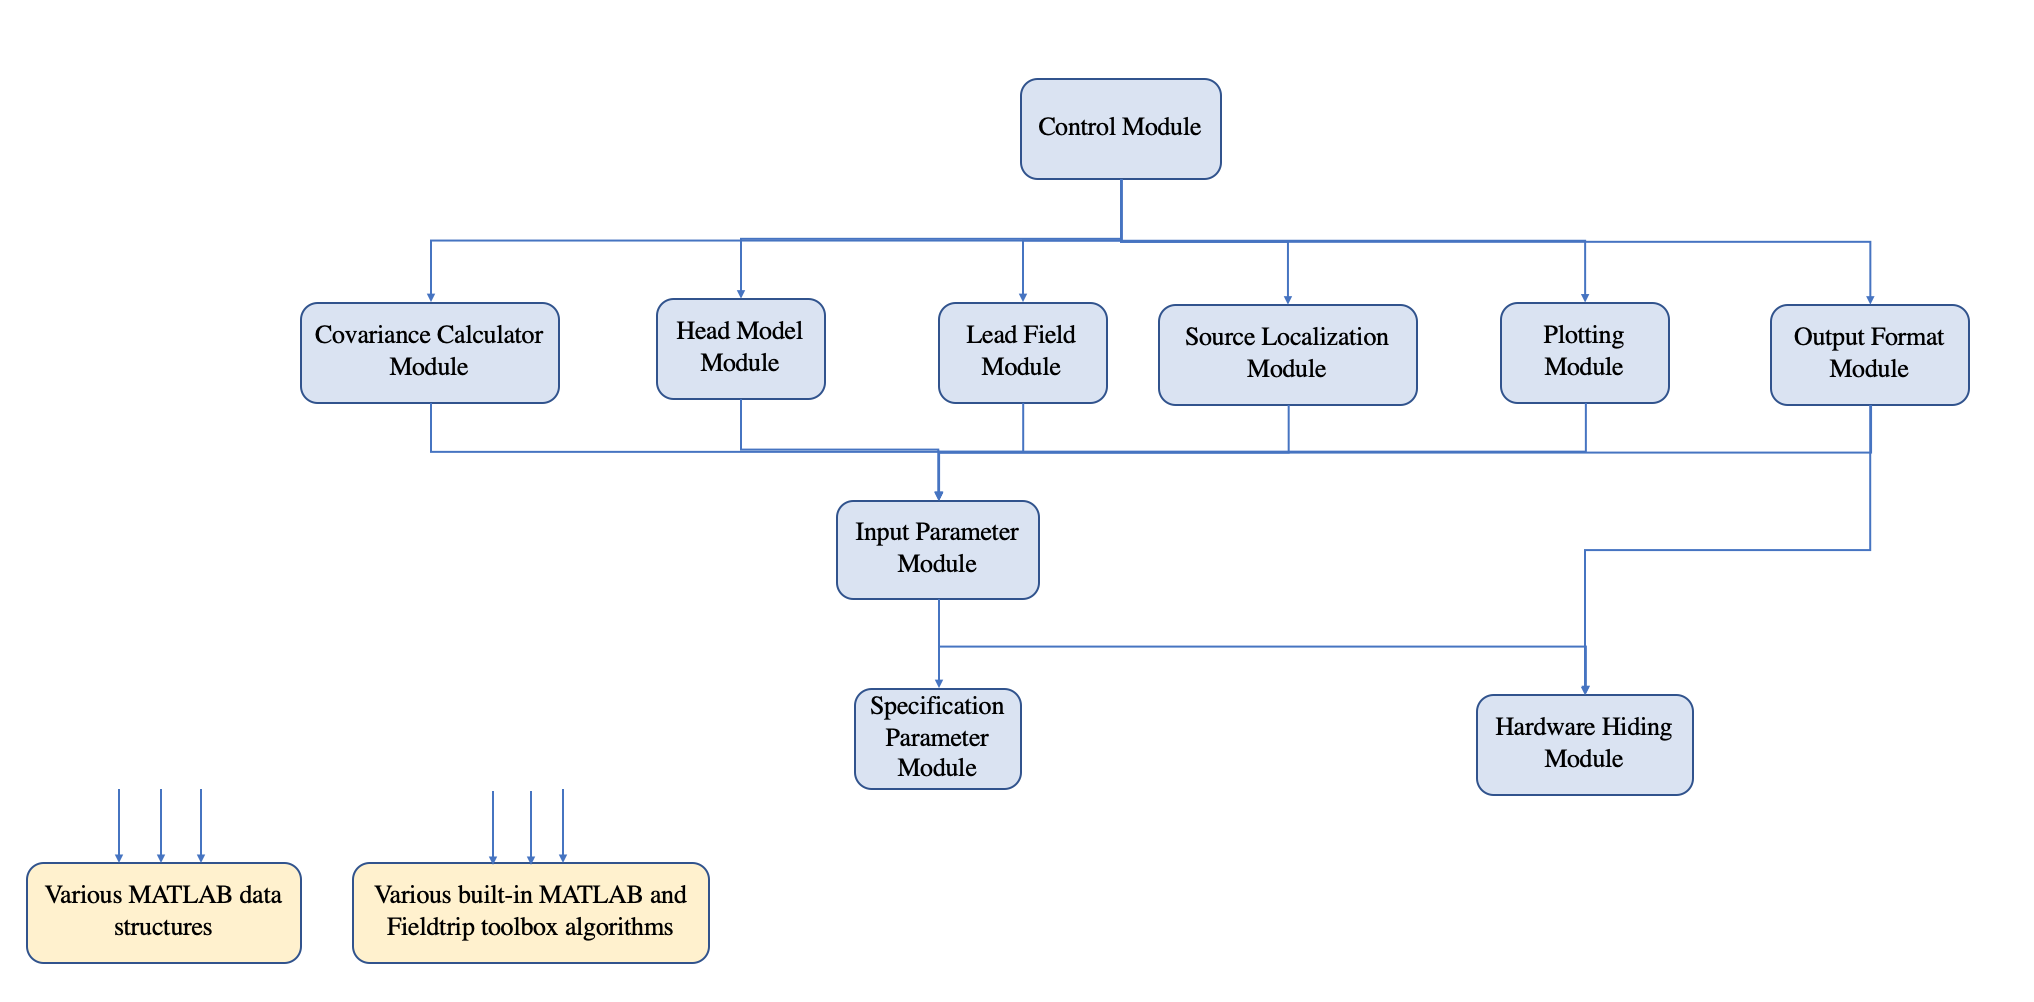
\includegraphics[width=1\textwidth]{UsesHierarchy.png}
\caption{Use hierarchy among modules}
\label{FigUH}
\end{figure}

%\section*{References}

\bibliographystyle {plainnat}
\bibliography{../../../refs/References}

\end{document}
